\documentclass{beamer}
\usepackage[utf8]{inputenc}
\usepackage[french]{babel}
\usepackage{amsmath}
\usepackage{amsfonts}
\usepackage{amssymb}
\usepackage{manfnt}
\usepackage{graphicx}
\usepackage{amsthm}
\usepackage{url}
\usepackage{makeidx}
\usepackage{mathtools}
\usepackage{dsfont}
\usepackage{hyperref}
\usepackage{float}
\usepackage{makeidx}
\makeatletter
\newcommand{\mathleft}{\@fleqntrue\@mathmargin0pt}
\newcommand{\mathcenter}{\@fleqnfalse}
\makeatother
\setlength\parindent{0pt}
\makeindex

\usetheme{Berlin}
\title{Modélisation et détection de délit d'initié}
\author{BROUX Lucas, HEANG Kitiyavirayuth}
\date{20 mars 2018}

\AtBeginSection[]{
  \begin{frame}
  \vfill
  \centering
  \begin{beamercolorbox}[sep=8pt,center,shadow=true,rounded=true]{title}
    \usebeamerfont{title}\insertsectionhead\par%
  \end{beamercolorbox}
  \vfill
  \end{frame}
}


% Prévoir 30 minutes de passage, 10 minutes de questions.

\begin{document}

%Title page
\begin{frame}
\titlepage
\end{frame}

\section*{Introduction}
\subsection*{Projet}
\begin{frame}
\frametitle{Présentation du projet}
\begin{itemize}
\item \textbf{Modélisation et détection de délit d'initié :}
\par Que se passe t'il lorsqu'un agent dispose d'une information confidentielle sur l'évolution future du marché ?
\item Objectifs :
	\begin{itemize}
	\item Analyser le gain de l'initié par rapport à un non-initié.
	\item Simuler la richesse de l'initié et du non-initié.
	\end{itemize}
\end{itemize}
\end{frame}

\subsection*{Choix du sujet}
\begin{frame}
\frametitle{Choix du sujet}
\begin{itemize}
\item Problématique concrète.
\item Aspect théorique : notions profondes et techniques.
\item Étude de cas particuliers possible à notre niveau.
\end{itemize}
\end{frame}

%Table of contents
\section*{Plan}
\begin{frame}
\frametitle{Plan de la présentation}
\tableofcontents
\end{frame}

%Sections MODELE DIFFUSIF 
\section{Modèle diffusif - cas particulier}

%SUBSECTION DESCRIPTIF DU MODELE 
\subsection{Description du modèle}

%EVOLUTION DES PRIX
\begin{frame}
\frametitle{Marché}
On considère 2 actions risquées sur le marché financier sur l'espace de probabilité $(\Omega, \mathcal{F}_t; t \in[0, T], \mathbb{P})$, dont les prix évoluent selon l'équation : 
\begin{equation*}
\begin{cases} 
S^0_t = S^0_0 +  \int_{0}^{t} S^0_s r_s ds \\
S^1_t = S^1_0 + \int_{0}^{t} S^1_s b^1_s ds + \int_{0}^{t} S^1_s \sigma^1_s dW_s, \quad 0 \leq t \leq T\\
S^2_t = S^2_0 + \int_{0}^{t} S^2_s b^2_s ds + \int_{0}^{t} S^2_s \sigma^2_s dW_s, \quad 0 \leq t \leq T
\end{cases}
\end{equation*}
\begin{itemize}
\item $W$ est un mouvement brownien à 2 dimensions dont $\mathcal{F}$ est la filtration naturelle.\\
\item Pour simplifier, on suppose que $b, r$ et $\sigma$ sont constants.
\end{itemize}
\end{frame}

\begin{frame}
\frametitle{Marché}
Les prix peuvent donc s'expliciter : 
\begin{displaymath}
\begin{cases}
S_t^0 &= S_0^0 e^{ r t } \\
S_t^1 &= S_0^1 e^{ \left( b_1 - \frac{1}{2} ||\sigma_1||^2 \right) t + \left( \sigma_1, W \left( t \right) \right) }  \\
S_t^2 &= S_0^2 e^{ \left( b_2 - \frac{1}{2} ||\sigma_2||^2 \right) t + \left( \sigma_2, W \left( t \right) \right) }
\end{cases}
\end{displaymath}

\end{frame}

%INITIE
\begin{frame}
\frametitle{Initié}
\begin{itemize}
\item On suppose qu'à $t= 0$, l'initié dispose a une information sur le futur, $L := \ln(S^1_T) - \ln(S^2_T)$, dont les autres investisseurs sur le marché ne disposent pas.  \\
\item Sa filtration naturelle est donc $\mathcal{Y}_t := \mathcal{F}_t \vee \sigma(L)$.\\
\item Il dispose d'un capital $X_0$ à $t=0$, consomme à une vitesse $c$, et il place la quantité $\theta^i$ sur l'actif $i$.\\
\item $\pi_t^i = \theta^i_t S^i_t$ : la somme investie sur le $i$-ième l'actif, $i= \{1, 2\}$.
\end{itemize}
\end{frame}

%HYPOTHESE D'AUTOFINACEMENT
\begin{frame}
\frametitle{Hypothèse d'autofinancement}
\begin{itemize}

\item Sa richesse au temps $t$ s'exprime donc : 
\begin{equation*}
X_t = \displaystyle \theta^0_t S^0_t  + \theta^1_t S^1_t  + \theta^2_t S^2_t - \int_{0}^{t} c_s ds
\end{equation*}

\item Nous supposons que son portefeuille est autofinançant : 
\begin{equation*}
dX_t = \displaystyle  \theta^0_t dS^0_t + \theta^1_t dS^1_t + \theta^2_t dS^2_t - c_t dt
\end{equation*}

\item En notant $R_t = (S^0_t)^{-1}$ le facteur d'actualisation, on obtient : 
\begin{equation*}
X_t R_t + \int_{0}^{t} R_s c_s ds = \int_{0}^{t} (R_s \pi_s, b_s - r_s \textbf{1})ds + \int_{0}^{t} (R_s \pi_s, \sigma_s dW_s)
\end{equation*}
\end{itemize}
\end{frame}


\subsection{Stratégie optimale}
\begin{frame}
\frametitle{Stratégie optimale}
\par L'initié cherche à optimiser son "utilité" :
\small
\begin{align*}
      J \colon &\underbrace{\mathcal{A}}_{\text{Stratégies admissibles}} \to \mathbb{R} \\
       &\left( \pi, c \right) \xmapsto{\phantom{\mathcal{A}}} J \left( X_0, \pi, c \right) := \mathbb{E} \left[ \int_0^A \log  \left( c_t \right) dt + \log \left( \underbrace{X_A^{\pi, c}}_{\text{Richesse au temps } A} \right) \left\vert\right. \mathcal{Y}_0 \right]
\end{align*}

\end{frame}

\begin{frame}
\frametitle{Stratégie optimale}

\begin{itemize}

\item où
\begin{displaymath}
\mathcal{A} = \left\lbrace \left( \pi, c \right), 
\begin{cases} 
\pi \enskip \mathcal{Y}-\text{prévisible}, \\
c > 0 \enskip \mathcal{Y}-\text{adapté}, \\ 
\int_0^T c_s ds < + \infty \enskip \text{et} \enskip \sigma^* \pi \in L^2 \left[ 0; T \right] \enskip \mathbb{P}-p.s., \\
X^{\pi, c} \geq 0 \enskip dt \otimes d \mathbb{P}-p.s. 
\end{cases}
\right\rbrace
\end{displaymath} 
\item $A < T$ : \emph{Temps final}.
\end{itemize}
\par Peut-on caractériser $\mathcal{A}$ sous une forme exploitable ?
\end{frame}


\subsection{Résolution du problème d'optimisation}
\begin{frame}
\frametitle{Raisonnement}
\begin{itemize}
\item La filtration de $W$ empèche le changement de probabilité pour se ramener à une mesure risque-neutre.
\item On va donc : 
\begin{itemize}
\item construire une probabilité $\mathbb{Q}$ pour laquelle $W$ est un $(\Omega, \mathcal{F}, \mathbb{Q})$-mouvement brownien.
\item construisons un nouveau mouvement brownien $B$ sur l'espace de probabilité filtré  $(\Omega, \mathcal{Y}, \mathbb{P})$ par la méthode de grossissement de filtration.\\
\item construire un mouvement brownien $\tilde{B}$ sur $(\Omega, \mathcal{Y}, \mathbb{Q}_1)$, avec $\mathbb{Q}_1$ probabilité risque-neutre sur $\mathcal{Y}$.
\end{itemize}
\end{itemize} 
\end{frame}

%\begin{frame}
%\frametitle{Changement de probabilités}
%\textbf{Proposition : } Sous hypothèses (techniques mais raisonnables), il existe une mesure de probabilité $\mathbb{Q}$ équivalente à $\mathbb{P}$ sur $\mathcal{Y}_A$, telle que pour $t \leq A$, $\mathcal{F}_t$ et $\sigma \left( L \right)$ sont $\mathbb{Q}$-indépendantes.
%\par En outre, $\left( W_t, t \leq A \right)$ est un $\left(\Omega, \mathcal{F}, \mathbb{Q} \right)$-mouvement brownien.
%\end{frame}

\begin{frame}
\frametitle{Grossissement de filtration}
\begin{itemize}
\item On a $L = \ln(S^1_T) - \ln(S^2_t)$
\begin{equation*}
= \underbrace{\ln ( \frac{S_0^1}{S_0^2} ) + ( ( b_1 - b_2 ) - \frac{1}{2} (||\sigma_1||^2 - ||\sigma_2|^2 ) ) T}_{=: \beta} + ( \underbrace{\sigma_1 - \sigma_2}_{=: \gamma}, W ( T ) ).
\end{equation*}
\item La loi conditionnelle de $L$ sachant $F_t$ suit donc une loi gaussienne $\mathcal{N} \left( \beta + \left( \gamma, W \left( t \right) \right), ||\gamma||^2 \left( T - t \right) \right)$
\item Donc $p \left( t, x \right) = \frac{1}{ ||\gamma|| \sqrt{2 \pi} \sqrt{T - t}} \underbrace{e^{-\frac{1}{2} \frac{\left( x - \beta - \left( \gamma, W \left( t \right) \right) \right)^2}{||\gamma||^2 \left( T - t \right)}}}_{ =: f \left( t, W \left( t \right) \right)}$
\end{itemize}
\end{frame}

\begin{frame}
\frametitle{Grossissement de filtration}
\begin{itemize}
\item On a montré que $p \left( t, x \right) = p \left( 0, x \right) + \int_0^t \left( \underbrace{ \frac{\left( x - \beta - \left( \gamma, W \left( t \right) \right) \right)}{||\gamma||^3 \sqrt{2 \pi} \left( T - t \right)^{\frac{3}{2}}} f \left( t, W \left( t \right) \right) \gamma}_{:= \alpha(s, x)}, dW \left( s \right) \right)$
\end{itemize}
\end{frame}


\begin{frame}
\frametitle{Grossissement de filtration}
\textbf{Propostion : } Sous hypothèses (techniques mais raisonnables), la loi conditionnelle de $L$ sachant $\mathcal{F}_t$ est absolument continue et il existe une version mesurable de la densité conditionnelle $(\omega, t, x) \mapsto p(\omega, t, x)$ qui est une $\mathcal{F}$-martingale et se représente par $ p(\omega, t, x) = p(0, x) + \int_{0}^{t}\alpha(\omega, s, x) dW_s$\

\end{frame}


\begin{frame}
\frametitle{Grossissement de filtration}
\textbf{Proposition : } Si $M$ est une $\mathcal{F}$-martingale locale continue égale à $ M_0 + \int_{0}^{t} \beta_s dW_s$, alors le crochet $d<M,P>_t$ est égal à $d<\alpha, \beta>_t dt$ et le processus $\tilde{M}_t = M_t + \int_{0}^{t}\frac{<\alpha(.,x),\beta>_u |_{x=L}}{p(u, L)} du$ est une $\mathcal{Y}$-martingale locale continue.
\begin{itemize}
\item En corollaire, le processus vectoriel $\Big(B_t = W_t - \displaystyle \int_{0}^{t} \frac{\alpha(u, L)}{p(u, L)} du, t \in [0, T[ \Big)$ est un mouvement brownien sur $(\Omega, \mathcal{Y}, \mathbb{P})$. 
\end{itemize}
\end{frame}

\begin{frame}
\frametitle{Grossissement de filtration}

On a donc construit un mouvement brownien $B$ sur l'espace probabilité filtré $(\Omega, \mathcal{Y}, \mathbb{P})$, qui est l'espace de probabilité de l'initié
\begin{equation*}
B_t = W_t - \displaystyle \int_{0}^{t} \underbrace{\frac{\left( \gamma, W \left( T \right) - W \left( u \right) \right) \gamma}{||\gamma||^2 \left( T - u \right)} }_{=:l(u, L)} du.
\end{equation*}

\end{frame}

\begin{frame}
\frametitle{Changement de probabilité}
\begin{itemize}
\item La forme de $l_t : = l(t, L)$ ne permet le changement de probabilité que sur $[0, A], A<T$ en non sur $[0, T]$. 
\item On introduit donc $\xi_t = -l_t - \eta_t$ où $\eta_t = (\sigma)^{-1} (b - r\textbf{1})$.
\end{itemize}

\end{frame}

\begin{frame}
\frametitle{Changement de probabilité}
\begin{itemize}
\item On peut vérifier que $\xi_t \in \mathbb{L}^2([0, T])$.
\item Soit $Y_t = e^{ \int_{0}^{t} \xi_s dB_s - \frac{1}{2} \int_{0}^{t} ||\xi_s||^2 d}$, une martingale exponentielle, alors $Z_T > 0$ p.s. et $\mathbb{E}_{\mathbb{P}} (Z_T) = Z_0 = 1$.\\
\item On peut donc appliquer le théorème de Girsanov qui nous dit que sous $\mathbb{Q}_1 = Y. \mathbb{P}$, 
\begin{equation*}
\tilde{B}_t = B_t - \displaystyle \int_{0}^{t}\xi_s ds
\end{equation*}
est un $(\mathcal{Y}, \mathbb{Q}_1)$ mouvement brownien.
\end{itemize}
%\textbf{Proposition : } Posons $M_t = e^{ \int_{0}^{t} \xi_s dB_s - \frac{1}{2} \int_{0}^{t} ||\xi_s||^2 d}$ pour $t \in [0,A] , A<T$. Alors $M$ est une $(

%\mathcal{Y}, \mathbb{P})$-martingale uniformément intégrable et, sous $\mathbb{Q}_1 = M.\mathbb{P}$, le processus

%\begin{center}
 
%$\tilde{B}_t = B_t - \displaystyle \int_{0}^{t}\xi_s ds$
 
%\end{center}

% est un $(\mathcal{Y}, \mathbb{Q}_1)$-mouvement brownien et les prix actualisés sont des $(\mathcal{Y}, \mathbb{Q}_1)$-martingales locales.
\end{frame}

\begin{frame}
\frametitle{Caractérisation de $\mathcal{A}$}
\begin{itemize}
\item Pour caracteriser $\mathcal{A}$, on introduit d'abord la \textit{stratégie de consommation-placement $(\pi, c)$ $ \mathcal{Y}$-admissible} qui rassure que la richesse finale $X^{\pi, c}$ pour la stratégie est toujours à valeurs positives ou nulles. .
\item Par propositions, on obtient 
\begin{equation*}
\mathcal{A} = \left\lbrace \left( \pi, c \right), \mathbb{E}_{\mathbb{Q}_1} \left[ X_A^{\pi, c} R_A + \int_0^A R_t c_t dt \left\vert\right. \mathcal{Y}_0 \right] \leq X_0 \right\rbrace .
\end{equation*}
\end{itemize}
\end{frame}

\begin{frame}
\frametitle{Résolution du problème d'optimisation}
Notre problème d'optimisation est donc 
\begin{equation*}
\mathbb{E}_{\mathbb{P}} \left[ \int_0^A \log  \left( c_t \right) dt + \log \left( X_A^{\pi, c}\right) \left\vert\right. \mathcal{Y}_0 \right]
\end{equation*}
sous contrainte 
\begin{equation*}
\mathbb{E}_{\mathbb{Q}_1} \left[ X_A^{\pi, c} R_A + \int_0^A R_t c_t dt \left\vert\right. \mathcal{Y}_0 \right] \leq X_0
\end{equation*}
\end{frame}

\begin{frame}
\frametitle{Résoltuion du problème d'optimisation}
Le problème se résout en utilisant la méthode des multiplicateurs de Lagrange :
\begin{align*}
\mathcal{L} &= \mathbb{E}_{\mathbb{P}} \big[ \int_{0}^{A} \log (c_t) dt + \log (X^{\pi, c}_A ) | \mathcal{Y}_0 \big] \\
&+ \lambda \Big( \mathbb{E}_{\mathbb{Q}_1} \big[ X^{\pi, c}_A R_A + \int_{0}^{A} R_t c_t dt | \mathcal{Y}_0 \big] - X_0 \Big)
\end{align*}

\end{frame}

\begin{frame}
\frametitle{Résolution du problème d'optimisation}
La solution du problème sont de la forme 
\begin{equation*}
\begin{cases} c^*_t = I_1 (\lambda^*Y_t R_t)\\
X^{\pi^*, c*}_A = I_2 (\lambda^* Y_A R_A)
\end{cases}
\end{equation*}
où $I_i(x) = ((\log(x))')^{-1} = \frac{1}{x}$ et $
\lambda^*$ est la solution de l'équation 
\begin{equation*}
\mathbb{E}_{\mathbb{P}} \Big[ \int_0^A R_t Y_t I_1(\lambda^* R_t Y_t)dt + R_A Y_A I_2(\lambda^* R_A Y_A ) | \mathcal{Y}_0 \Big] = X_0.
\end{equation*}
$ \Leftrightarrow \lambda^* = \frac{X_0}{A +1}$.
\end{frame}

\begin{frame}
\frametitle{Résolution du problème d'optimisation}
On obtient donc
\begin{equation*}
\begin{cases}
R_t c_t^* &= \frac{X_0}{A + 1} \frac{1}{Y} \left( t \right) \\
R_t X_t^* &= \frac{X_0 \left( A + 1 - t \right)}{A + 1} \frac{1}{Y} \left( t \right)
\end{cases}
\end{equation*}
où : 
\begin{displaymath}
Y \left( t \right) = 
\begin{cases}
e^{- \int_{0}^{t} \left( \eta_s, dW_{s} \right)-\frac{1}{2} \int_{0}^{t} {\| \eta_s \|}^{2} ds} & \text{pour le non initié} \\
e^{- \int_{0}^{t} \left( l_{s} + \eta_s, dB_{s} \right) - \frac{1}{2} \int_{0}^{t} {\| l_{s} + \eta_s \|}^{2} ds} & \text{pour l'initié}
\end{cases}
\end{displaymath}
\end{frame}
\subsection{Analyse du gain de l'initié}

\begin{frame}
\frametitle{Forme explicite du gain}
\par On a :
\begin{displaymath}
Y \left( t \right) = 
\begin{cases}
e^{- \left( \eta, W_{t} \right)-\frac{1}{2} t {\| \eta \|}^{2}} =: Y_0 \left( t \right) & \text{pour le non initié} \\
e^{- \int_{0}^{t} \left( l_{s} + \eta, dW_{s} - l_s ds \right) - \frac{1}{2} \int_{0}^{t} {\| l_{s} + \eta \|}^{2} ds} & \text{pour l'initié}
\end{cases}
\end{displaymath}

\par On s'intéresse au gain de l'initié par rapport au non-initié : 

\begin{displaymath}
	\begin{split}
	Z \left( t \right) &:= \frac{Y_0 \left( t \right)}{Y \left( t \right)} = \frac{ e^{- \left( \eta, W_{t} \right)-\frac{1}{2} t {\| \eta \|}^{2}}}{e^{- \int_{0}^{t} \left( l_{s} + \eta, dW_{s} - l_s ds \right) - \frac{1}{2} \int_{0}^{t} {\| l_{s} + \eta \|}^{2} ds}} \\
	&= e^{ \int_{0}^{t} \left[ \left( l_s, dW_{s} \right) ds \right] - \frac{1}{2} \int_{0}^{t} {\| l_{s} \|}^{2} ds}
	\end{split}
\end{displaymath}
\end{frame}
 
\begin{frame}
\frametitle{Forme explicite du gain}
\par Donc
\begin{displaymath}
d \log \left( Z \left( t \right) \right) = \underbrace{\left(l_s, d W_s \right)}_{ = \frac{d p \left( t, L \right)}{p \left( t, L \right)}} - \frac{1}{2} {\| l_{s} \|}^{2} ds = d \log \left( p \left( t, L \right) \right)
\end{displaymath}

\par Donc $\frac{Z \left( t \right)}{ p \left( t, L \right) }$ est constant :

\begin{displaymath}
	\begin{split}
	Z \left( t \right) &= \frac{Z \left( 0 \right)}{ p \left( 0, L \right) } p \left( t, L \right)
	\end{split}
\end{displaymath}
\par Interprétation : pour tout $t$, le gain proportionnel de l'initié correspond - à une constante initiale près -  à la densité conditionnelle de la variable $L$ sachant $\mathcal{F}_t$, prise en $x = L$.
\end{frame}
 
\begin{frame}
\frametitle{Forme explicite du gain}
\par On obtient donc :
\begin{displaymath}
	\begin{split}
		\boxed{
	Z \left( t \right) = \frac{\sqrt{T}}{\sqrt{T - t}} e^{\frac{- \left( \gamma, W \left( T \right) - W \left( t \right) \right)^2}{2 ||\gamma||^2 \left( T - t \right)} + \frac{\left( \gamma, W \left( T \right) \right)^2}{2 ||\gamma||^2 T }}
		}
	\end{split}
\end{displaymath}
\par En remplaçant $ \left( \gamma, W \left( T \right) - W \left( t \right) \right)^2 $ par son espérance $||\gamma||^2 \left( T - t \right)  $,

\begin{displaymath}
	Z \left( t \right) \simeq \frac{\sqrt{T}}{\sqrt{T - t}} \quad \substack{\text{\textdbend raisonnement heuristique, } \\ \text{ n'est pas une estimation de } \mathbb{E} \left[ Z \left( t \right) \right]}
\end{displaymath}

\end{frame}

\begin{frame}
\frametitle{Analyse du gain}

\par Cela fournit un minorant (via $e^x \geq 1 + x$) :
\begin{displaymath}
Z \left( t \right) \geq  \frac{\sqrt{T}}{\sqrt{T - t}} \left( 1 + \left( \underbrace{\frac{- \left( \gamma, W \left( T \right) - W \left( t \right) \right)^2}{2 ||\gamma||^2 \left( T - t \right)} + \frac{\left( \gamma, W \left( T \right) \right)^2}{2 ||\gamma||^2 T }}_{\mathbb{E} \left[ \cdot \right] = 0} \right) \right)
\end{displaymath}

\par Donc
\begin{displaymath}
\mathbb{E} \left[ Z \left( t \right) \right] \geq  \frac{\sqrt{T}}{\sqrt{T - t}} \xrightarrow[t \to T]{} + \infty
\end{displaymath}
\end{frame}

\begin{frame}
\frametitle{Visualisation}
\par Moyenne de 100 simulations de $Z$ (\emph{simulations\_averages.py}) : 
\begin{figure}[H]
  \centering
    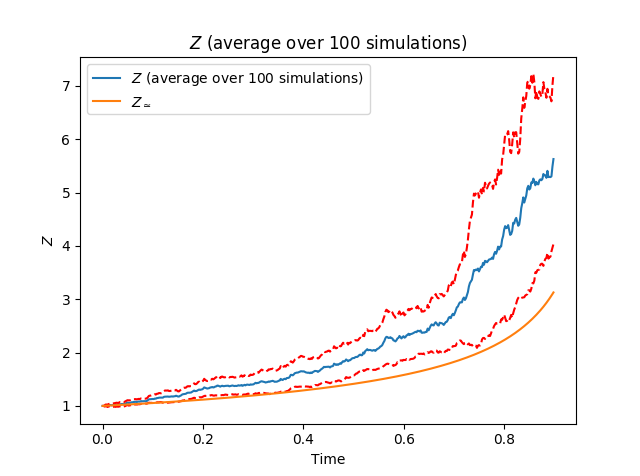
\includegraphics[width=0.7\textwidth]{images/average_100.png}
  \caption{}
\end{figure}
\end{frame}

\begin{frame}
\frametitle{Visualisation}
\par Moyenne de 1000 simulations de $Z$ (\emph{simulations\_averages.py}) : 
\begin{figure}[H]
  \centering
    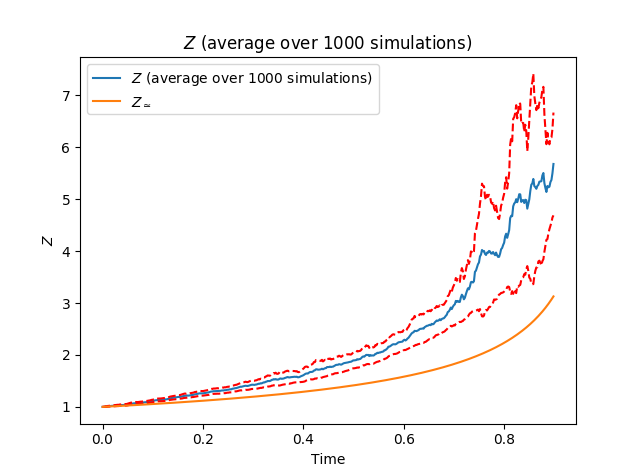
\includegraphics[width=0.7\textwidth]{images/average_1000.png}
  \caption{}
\end{figure}
\end{frame}

\begin{frame}
\frametitle{Visualisation}
\par Moyenne de 10000 simulations de $Z$ (\emph{simulations\_averages.py}) : 
\begin{figure}[H]
  \centering
    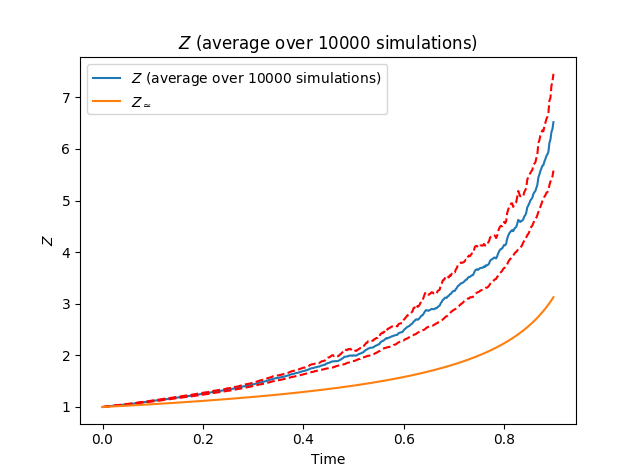
\includegraphics[width=0.7\textwidth]{images/average_10000.png}
  \caption{}
\end{figure}
\end{frame}

\subsection{Simulations}

\begin{frame}
\frametitle{Simulations}
\par Nous avons implémenté numériquement les formules (\emph{repository Github} du projet : \url{https://github.com/lucas-broux/Projet-3A}).
\begin{figure}[H]
  \centering
    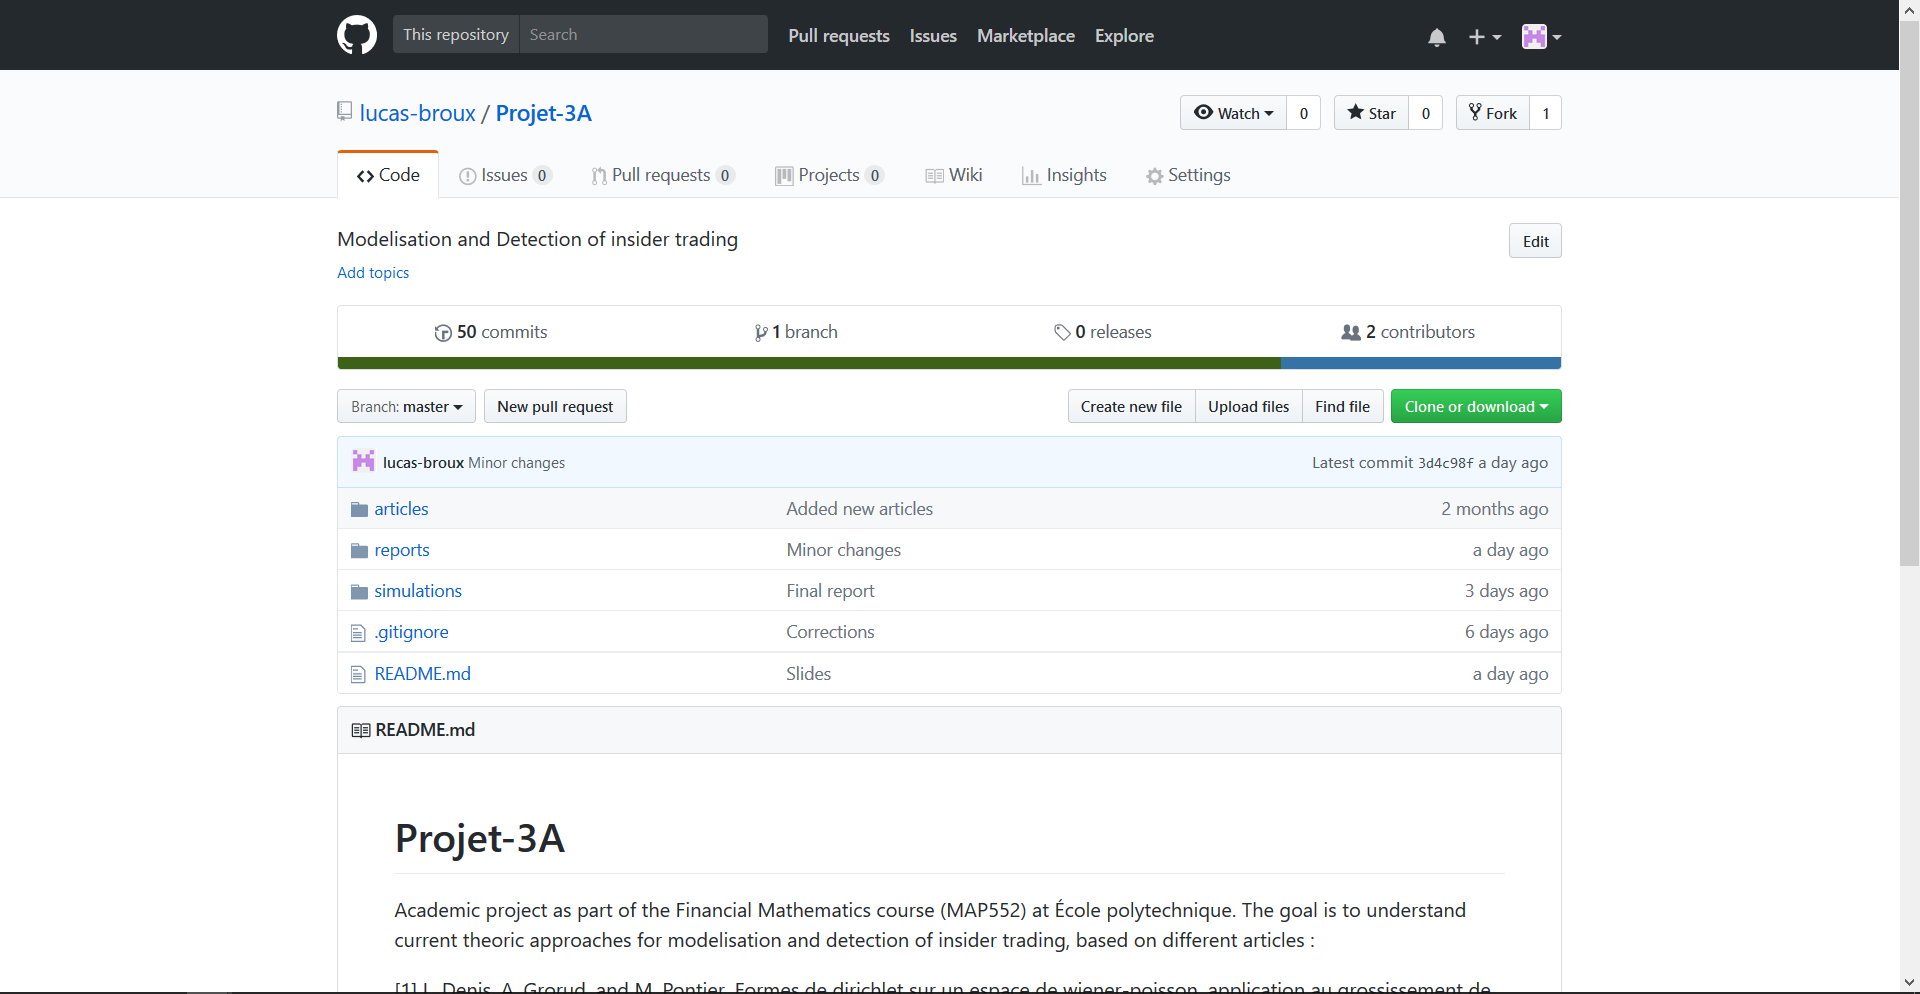
\includegraphics[width=0.7\textwidth]{images/github.png}
  \caption{}
\end{figure}

\end{frame}

\begin{frame}
\frametitle{Simulations}

\end{frame}

\begin{frame}
\frametitle{Simulations}

\end{frame}

\begin{frame}
\frametitle{Simulations}

\end{frame}

\section{Modèle avec sauts}
\subsection{Description du modèle}

\begin{frame}
\frametitle{Marché}
On considère $d$ actions risquées sur le marché sur l'espace de probabilité $(\Omega, \mathcal{F}_t; t\in [0, T], \mathbb{P})$. Les prix des actions, dirigés par un mouvement brownien $W$ de dimension $m$ et un processus de Poisson $N$ de dimension $n$, qui produit des sauts, ont pour équation :
\begin{align*}
\begin{cases}
S^0_t &= S_0^0 + \int_{0}^{t} S^0_s r_s ds \\
S_t^i &= S_0^i + \int_{0}^{t}S_s^i b_s^i ds + \int_{0}^{t}S_s^i \sigma^{ij}_t \sum_{j = 1}^{d} d(W^*, N^*)^{*}_j(s) \end{cases}
\end{align*}
$ 0 \leq t \leq T, i = 1, ..., d, m+n = d$
\end{frame}

\subsection{Raisonnement}

\begin{frame}
\frametitle{Raisonnement}
\begin{itemize}
\item On adapte les informations et le comportement de l'initié décrits dans le marché diffusif. 
\item L'initié cherche à optimiser la fonction 
\begin{equation*}
\mathbb{E}_{\mathbb{P}} \Big[ \displaystyle \int_{0}^{A} \log (c_t)dt + \log(X_A^{\pi, c})\Big |\mathcal{Y}_0\Big]
\end{equation*}
dans l'ensemble de toutes les stratégies admissibles.
\item Les méthodes dans le marché diffusif s'appliquent pour ce marché aussi pour faire grossir la filtration et se ramener à une mesure risque-neutre sur $(\Omega, \mathcal{Y}, \mathbb{Q}_1)$.
\end{itemize}
\end{frame}

\subsection{Résolution du problème d'optimisation}
\begin{frame}
\frametitle{Résolution du problème d'optimisation}
Le problème d'optimisation 
\begin{equation*}
\mathbb{E}_{\mathbb{P}} \Big[ \displaystyle \int_{0}^{A} \log (c_t)dt + \log(X_A^{\pi, c})\Big |\mathcal{Y}_0\Big]
\end{equation*}
sous contrainte 
\begin{equation*}
\mathbb{E}_{\mathbb{Q}_1} \left[ X_A^{\pi, c} R_A + \int_0^A R_t c_t dt \left\vert\right. \mathcal{Y}_0 \right] \leq X_0
\end{equation*}
a pour solutions : 
\begin{displaymath}
\text{pour } t \in [0, A], \quad \begin{cases}
 R_t {c}_t^* &= \frac{X_0}{A+1} \frac{1}{Y}(t)\\
 R_t {X}_t^* &= \frac{X_0(A+1-t)}{A+1}\frac{1}{Y}(t)\\
 {\pi}_t^* &= (\sigma^*_t)^{-1}\frac{Y(t)}{Y(t^{-1})}\widehat{X}_t l_t
\end{cases}
\end{displaymath}
\end{frame}

\begin{frame}
\frametitle{Résolution du problème d'optimisation}
\begin{itemize}
\item avec $Y(t) = Y_0(t) / Z(t)$, la relation liant la stratégie optimale de l'initié ($Y(t)$) avec celle du non initié ($Y_0(t)$)\\
\item $Z$ est la densité conditionnelle de $L$ sachant $\mathcal{F}_t$, prise en $x = L$,
\item $Y_0 = \varepsilon \left(\displaystyle \int_{0}^{\cdot} \left(- \left( \eta_W \left( s \right), dW_s \right) + \left( - \eta_M \left(  s \right) - I_n, dM_s \right) \right)\right)$, où
\begin{itemize}
\item[•] $\eta_W \left( t \right) := m$ premières lignes de $(\sigma_t)^{-1}(b_t - r_t I_d)$.\
\item[•] $ \eta_M \left( t \right)$ est un processus de dimension $n$, dont les composants sont supposés positifs, tel que $q_t. \kappa_t := n$ dernières lignes de $(\sigma_t)^{-1}(b_t - r_t I_d)$.
\end{itemize}
\end{itemize}
\end{frame}

\section{Conclusion}

\begin{frame}
\frametitle{Conclusion}
\begin{itemize}
\item Il est possible d'exprimer et d'étudier le gain de l'initié dans des cas plus ou moins particuliers.
\item Des théorèmes généraux mais techniques assurent que - sous hypothèses - le raisonnement reste vrai.
\item Simulations numériques possibles dans certains cas, mais rendues difficiles dans d'autres.
\end{itemize}
\end{frame}

\section{Retour d'expérience}

\begin{frame}
\frametitle{Retour d'expérience}
\begin{itemize}
\item Travail de lecture d'article :
	\begin{itemize}
	\item Identifier les passages trop techniques.
	\item Étudier en détail les cas particuliers.
	\end{itemize}
\item Travail en binôme.
\end{itemize}
\end{frame}


\begin{frame}
\Huge \center Merci !
\huge\center Questions ?
\end{frame}


\begin{frame}
\end{frame} % to enforce entries in the table of contents


\end{document}